\cleardoublepage
\chapter{Results}
%\label{ch:chapter1}
\label{makereference}
\section{Reconfigurable platform}
The architecture described in the previous section has been implemented using the VHDL language. To test its correct operation, the Vivado environment and the Virtex 690T FPGA have been used. Although it is not a radiation-protected FPGA, the architecture of this algorithm is scalable so that its adaptation to other sensor sizes or FPGAs should not be a problem.

\begin{center}
 \begin{tabular}{|c|c|c|c|c|c|} 
 \hline
 Part number & Slices & Logic cells & Flip-Flops & BRAM & DSP Slices \\
 \hline
 XCE7VX690T & 108,300 & 693,120 & 866,400 & 1,470Kb & 3,600\\
 \hline
\end{tabular}
\end{center}

\section{Hyperpectral image datasets}
Two hyperspectral images have been used for the work, one taken by the HYDICE sensor and the other by the AVIRIS sensor. Both images are commonly used as reference in hyperspectral applications. 
\\
In the field of the scene captured by HYDICE, 15 panels of different sizes were placed in a 3 x 5 meter configuration. The following images show the false color image and the location of the panels as detected by commercial software.
\begin{figure}[!ht]
    \begin{tabular}[b]{c|c}\hline
      Horizontal res & 64 \\ \hline
      Vertical res & 64 \\ \hline
      Bands & 210 \\ \hline
      Spectral res & 400 - 2500nm \\ \hline
      Spatial res & 1,56meter/pixel \\ \hline
      Size & 1,6 MB\\ \hline
    \end{tabular}
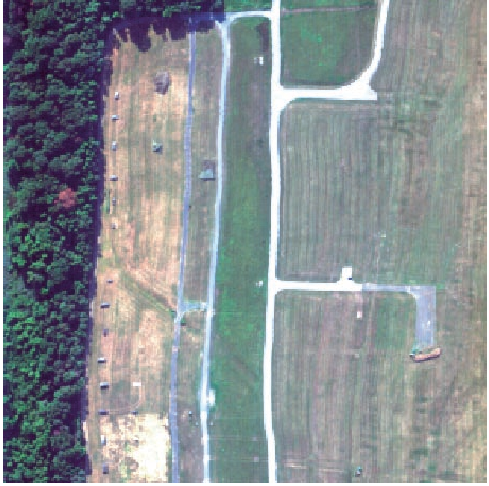
\includegraphics[height=1.5in]{figures/hydice_bad.png}
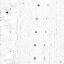
\includegraphics[height=1.5in]{figures/hydice_rx.png}
    \caption{Hydice sensor information and image in false color}
  \end{figure}
  %https://www.indexdatabase.de/db/s-single.php?id=84
\\
\\
The image taken by the AVIRIS sensor was taken on September 16, 2001, five days after the terrorist attacks that brought down the WTC towers and its surrounding buildings. The spatial resolution of this image is very high because a very low altitude flight was performed. Along with the false color image, an image with the anomalies detected by a commercial program surrounded to indicate their position is provided.
\begin{figure}[!ht]
    \begin{tabular}[b]{c|c}\hline
      Horizontal res & 614 \\ \hline
      Vertical res & 512 \\ \hline
      Bands & 224 \\ \hline
      Spectral res & 360 - 2500nm \\ \hline
      Spatial res & 1,7meter/pixel \\ \hline
      Size & 140 MB\\ \hline
    \end{tabular}
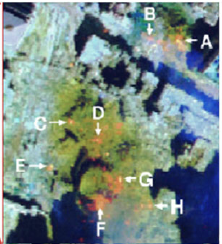
\includegraphics[height=1.5in]{figures/wtc_bad.png}
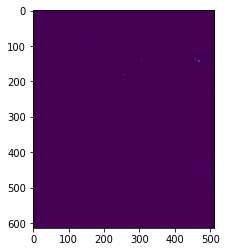
\includegraphics[height=1.5in]{figures/wtc_rx.png}
    \caption{Aviris sensor sensor information and image in false color}
  \end{figure}
  %https://www.indexdatabase.de/db/s-single.php?id=28
\\
\\
\section{Adequacy of approximation}
\subsection{Floating point}
The results provided by the floating point version of this system are the same as those provided by the equivalent software version, so it can be considered valid.

\subsection{Fixed point}
The fixed point version of the system is an approach to the floating point system with the intention of maintaining the highest possible accuracy with limited use of resources.
Therefore, the results are different and an assessment of their accuracy must be made. For this purpose, three metrics have been used.
\\
\\
In the first and simplest, it has been verified that the amount of detected anomalies can be found in the first x positions in both results, regardless of the order.
\\
\\
Extending the previous strategy, it has been checked for the non coinciding elements, if any neighbor has been detected in the environment. A neighbor is defined as an adjacent pixel, both in a straight line and in diagonal.
\\
\\
Finally, the first strategy has been extended again, this time it has been checked if for the non coincidences an anomaly with a spectral similarity of less than 5 degrees has been found.
\\
%https://www.harrisgeospatial.com/docs/SpectralAngleMapper.html
\paragraph{Spectral similarity}
The Spectral Angle Mapper (SAM) is a physics-based spectral classification that uses an n-D angle to match pixels with reference spectra. The algorithm determines the spectral similarity between two spectra by calculating the angle between the spectra and treating them as vectors in a space with a dimensionality equal to the number of bands. This technique, when used in calibrated reflectance data, is relatively insensitive to the effects of illumination and albedo.
\begin{figure}[h!]
\begin{minipage}[t]{0.5\linewidth}
\centering
\[\alpha = \cos^{-1}\left ( \frac{\sum\limits^{nb}_{i=1}{t_{i}r_{i}}}{\left ( \sum\limits^{nb}_{i=1}{t_{i}^2} \right )^{1/2}\left ( \sum\limits^{nb}_{i=1}{r_{i}^2} \right )^{1/2}} \right )\]
\label{sam}
\end{minipage}
\begin{minipage}[t]{0.05\linewidth}
\end{minipage}
\begin{minipage}[t]{0.45\linewidth}
\vspace{0.7cm}
$\alpha$ = spectral angle between vectors
\\
nb = number of spectral bands
\\
t = target pixel
\\
r = reference pixel
\end{minipage}
\caption{Spectral Angle Mapper algorithm.}
\end{figure}

In the results of HYDICE it can be seen that if a pixel is not the one detected, neither is it a neighboring pixel, but that all the results correspond according to their spectral signature. This is because of the large size of the targets to detect, where there are several pixels in the same target and the order of detection may vary. However, as the pixels in each target are spectrally similar, the signature always matches. The image is therefore quite easy to analyze and good results have been achieved.
\begin{figure}[!ht]
	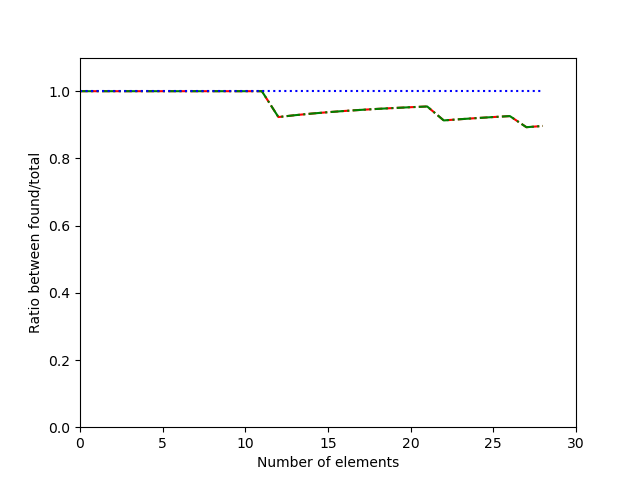
\includegraphics[height=2.0in]{figures/hydice.png}
	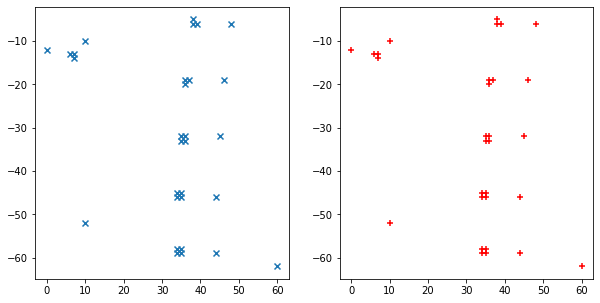
\includegraphics[height=2.0in]{figures/hydice_res.png}
\end{figure}

The WTC image is more complex and it can be seen that the detection of exact pixels and neighbors quickly falls. However, the spectral signatures match for the most part, especially considering the number of real hot spots found in the image. Therefore the results can also be taken as successful.
\begin{figure}[!ht]
	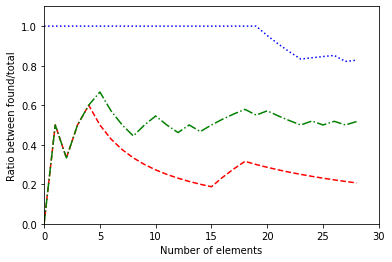
\includegraphics[height=2.0in]{figures/wtc.png}
	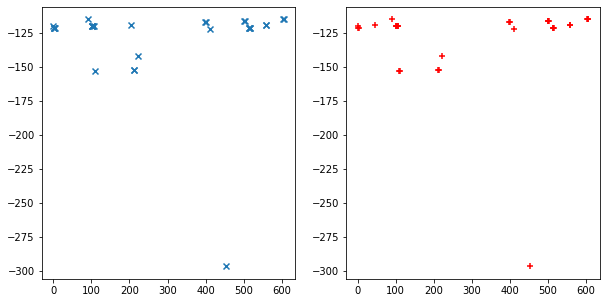
\includegraphics[height=2.0in]{figures/wtc_res.png}
\end{figure}

It should be noted that the shift values within the calculations have been adapted for each image with the intention of detecting the greatest number of anomalies possible, so that the results obtained in a real system will be slightly lower. Even so, the values between the two images are quite similar, despite the great difference between the data they represent.
\\
In addition, since it is a reconfigurable system, these values can be modified after the system is put into operation, both to accept a wider range of images, and to obtain more accurate results.

nota: tengo que incluir una leyenda
nota: tengo que pintar bien las imágenes para averigüar que estoy analizando realmente y poder hacer una mejor valoración de los resultados

\section{Computational efficiency}
When evaluating performance, both the resources used and the processing time must be assessed. These data are given both in those obtained for the two sensors and according to their characteristics, more specifically number of bands and pixels.
\\
It should be noted that performance data has been obtained by ignoring the input and output of data, which is often the bottleneck in this type of system.
\\

A comparison of resource expenditure per module, which is closely related to its complexity in time, is also provided.

\begin{center}
 \begin{tabular}{|c|c|c|c|c|} 
 \hline
 Module & LUT & Register & BRAM & DSP \\ [0.5ex] 
 \hline\hline
 Inverse & $410*bands+3484$ & $316*bands+10427$ & $<bands$ & $10*bands$\\ 
 \hline
 Mean subtraction & $bands+41$ & $136$ & $0$ & $1$\\ 
 \hline
 Matrix multiplication & $80*bands+75$ & $91*bands+223$ & $pixels/64$ & $4*bands$\\ 
 \hline
 Sort results & $186$ & $176$ & $0$ & $0$\\ 
 \hline
\end{tabular}
\end{center}

\begin{center}
 \begin{tabular}{|c|c|} 
 \hline
 Stage & Latency \\ [0.5ex] 
 \hline\hline
 Inverse & $\mathcal{O}(bands+bands^2) = \mathcal{O}(bands^2)$\\ 
 \hline
 Mean subtraction & $\mathcal{O}(1)$\\
 \hline
 Matrix multiplication & $\mathcal{O}(bands*pixels+bands)$\\
 \hline
 Sort results & $\mathcal{O}(2*bands) = \mathcal{O}(bands)$\\
 \hline
\end{tabular}
\end{center}

Nota: aquí me falta alguna cosilla.
Finally, the total resource utilization and the time and frequency specifications provided by Vivado are also stated:
\begin{center}
 \begin{tabular}{|c|c|c|c|c|} 
 \hline
 Resource & Hydice & Aviris\\ [0.5ex] 
 \hline\hline
 periodo & 0 & 0\\ 
 \hline
 frecuencia & 0 & 0\\ 
 \hline
 setup & 0 & 0\\ 
 \hline
 hold & 0 & 0\\ 
 \hline
\end{tabular}
\end{center}